\documentclass[a4paper,12pt]{article}
\usepackage{hyperref}
\usepackage{graphicx}
\graphicspath{ {./images/} }
\usepackage{geometry}

%\usepackage[margin=1in]{geometry}

\newcommand{\teamnr}{6}
\newcommand{\datum}{\today}
\newcommand{\coordinator}{Said Yandarbiev}

\title{\textbf{Programming Project Databases \\ Database diagram Team \teamnr}}
\author{Jorden Van Handenhoven\and Mohammed Shakleya\and Said Yandarbiev\and Sam Roggeman\and William Steklein}


\begin{document}
		
	\maketitle
	
		
	
	\tableofcontents
	\pagebreak
	\newgeometry{top=20mm,bottom=10mm,left = 10mm, right=10mm}
	\section{Introduction}
	To make our database diagram we used datagrip, we also used datagrip to make a diagraph from our sql-input. Our full diagram below.\\ 
	\begin{center}
  		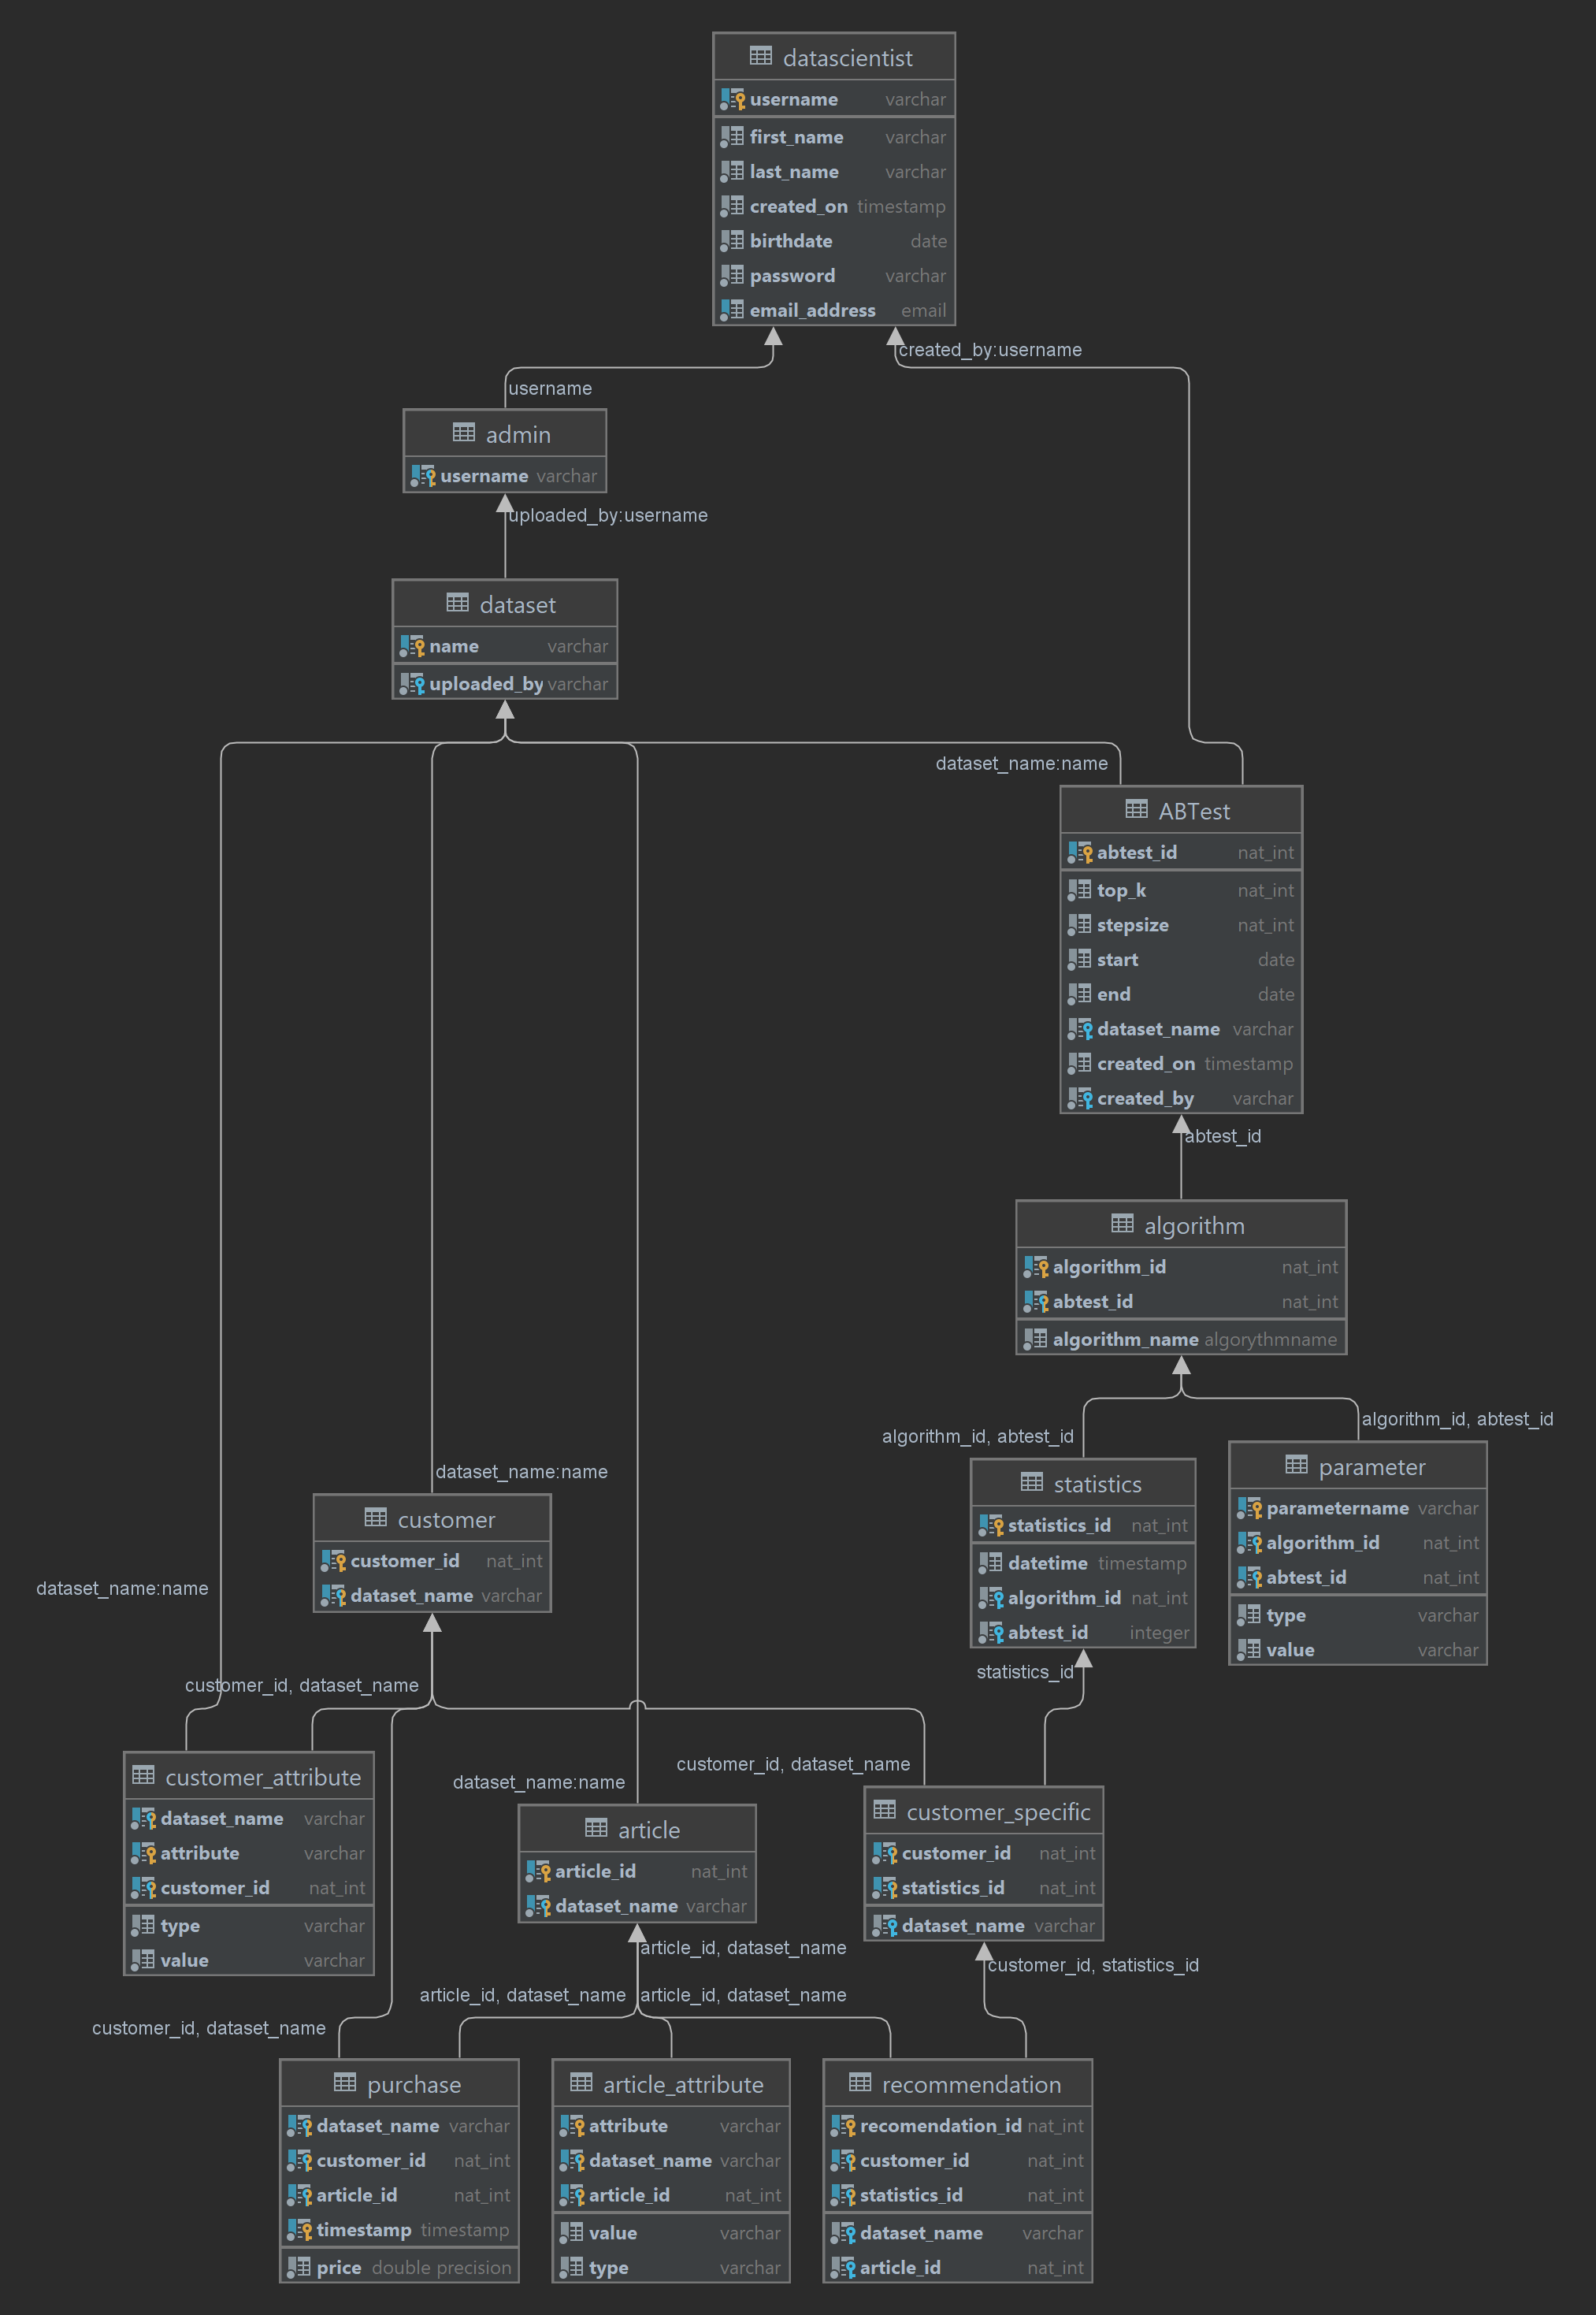
\includegraphics[height=600px]{FullDiagraph.png}
\end{center}
\restoregeometry     
	\pagebreak
	\section{Users}
	\subsection{datascientist}
	First we have the datascientist which all have a unique username (PK). They can log in onto the site and create ABTests, view their history and look at the datasets. Every user has a first and last name, creation date of the account, birth-date and password.
	\begin{center}
	\subsection{Admin}
	An admin has a 'isa' relationship with a datascientist. An admin s the only one who can upload datasets of purchases, customers and articles. Admin is connected through a foreign key to datascientist, which is also it's only field and it's primary key.
		  		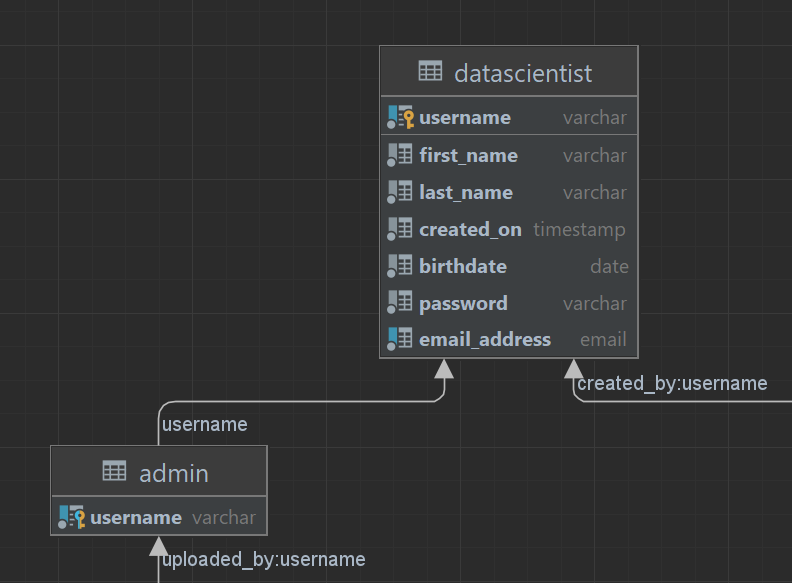
\includegraphics[width=\textwidth]{Users.png}
	\end{center}
	\pagebreak
	\section{Dataset}
	A dataset has a dataset-name as primary key. It is connected to an admin through a foreign key "uploaded-by" as only admins can upload such a set.
	\begin{center}
		  		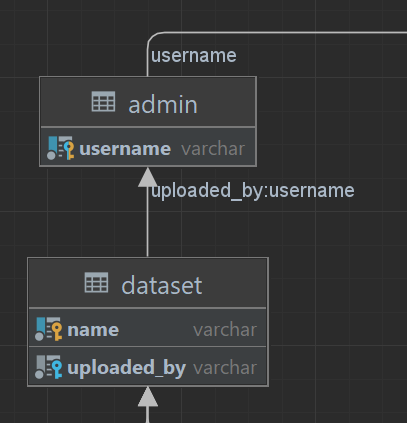
\includegraphics[width=\textwidth]{Dataset.png}
	\end{center}
	\pagebreak
	\subsection{Customers}
	A customer is a weak entity of a dataset, it's primary key is composed of a dataset-name (foreign key to dataset) and a customer-id to differentiate between customers in a given dataset = PK[dataset-name, customer-id].
	\subsubsection{Customer-Attribute}	
	Customer Attribute is where we store the actual (dynamic) data of a customer. It is a weak entity of customer and therefore contains a foreign key to a customer (customer-id, dataset-name). On top of this foreign key, the "attribute" is added which is the name of the field/attribute. So the final primary/composite key is (customer-id, dataset-name, attribute). It has a type and a value so it can be used as intended.
	
	\begin{center}
		  		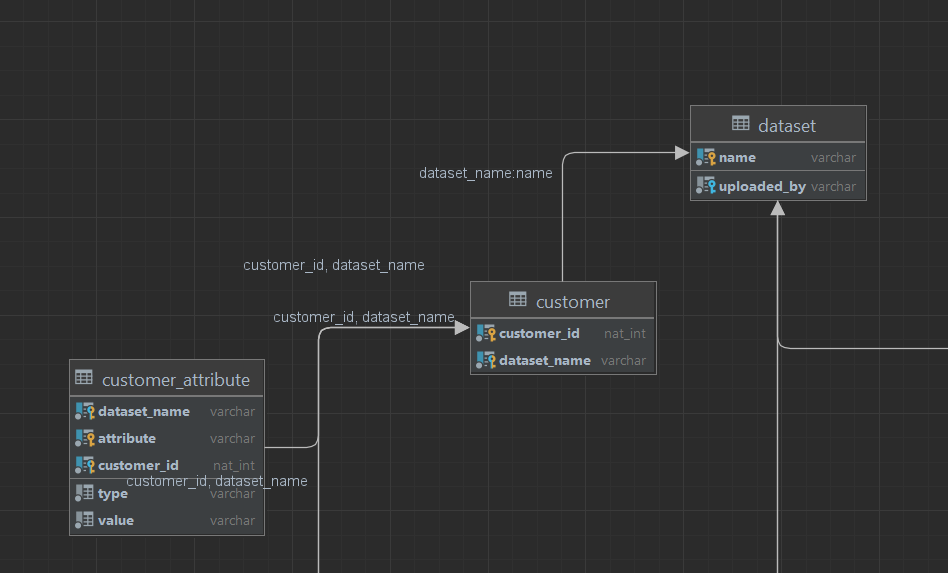
\includegraphics[width=\textwidth]{Customer.png}
	\end{center}
	\pagebreak
	\subsection{Articles}
		An Article is a weak entity of a dataset, it's primary key is composed of a dataset-name (foreign key to dataset) and an article-id to differentiate between articles in a given dataset = PK[dataset-name, article-id].
		\subsubsection{Article-Attribute}
			Article Attribute is where we store the actual (dynamic) data of an article. It is a weak entity of article and therefore contains a foreign key to an article (article-id, dataset-name). On top of this foreign key, the "attribute" is added which is the name of the field/attribute. So the final primary/composite key is (article-id, dataset-name, attribute). It has a type and a value so it can be used as intended.
	\begin{center}
		  		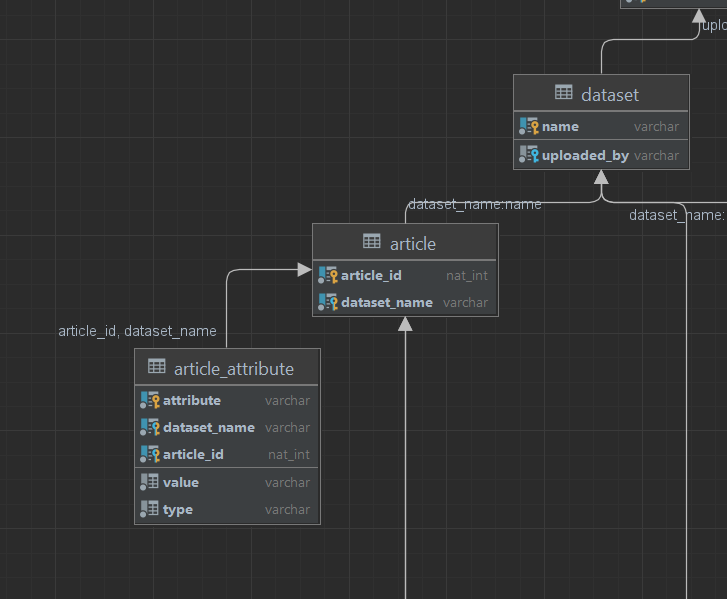
\includegraphics[width=\textwidth]{Article.png}
	\end{center}
	\pagebreak	
	\subsection{Purchases}
	A purchase is defined by a person with "customer-id" buying an article with "article-id" belonging to the same dataset on "timestamp" for the price "price". Therefore the primary key of a purchase is (article-id,customer-id, dataset-name, timestamp). The price at the time of purchase is kept in an extra field. It references to customer(customer-id, dataset-name ) and article(article-id, dataset-name ), with the same dataset-name in both references.
		\begin{center}
		  		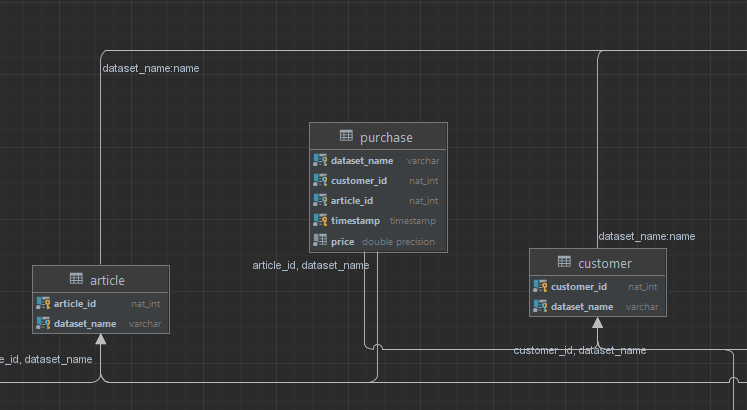
\includegraphics[width=\textwidth]{Purchase.png}
	\end{center}
	\pagebreak	
	\section{ABTest}		
	An abtest has a unique id [PK], It contains the test-wide parameters namely top-k, stepsize,start,end and dataset-name which references dataset(dataset-name). It's creator is kept in "uploaded-by" which references a datascientist. And it's creation time is also kept which defaults to now().
			\begin{center}
		  		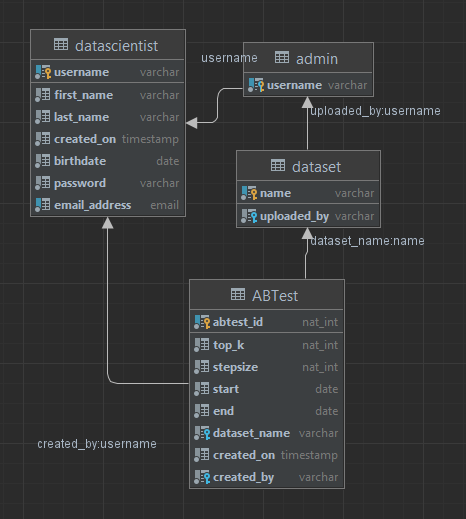
\includegraphics[width={250px}]{ABTest.png}
	\end{center}
	
	\subsection{Algorithm} An algorithm itself is a weak entity and belongs to an abtest(abtest-id). It's own primary key is (algorithm-id,ABTest-id). It also contains the name of the algorithm (this is so that we can identify which exact algorithm we have to execute). We can make multiple algorithms and link them to the same ABTest.
\begin{center}

		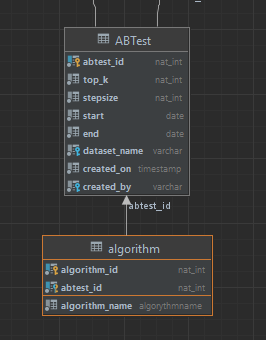
\includegraphics[height={200px}]{Algorithm.png}
	
\end{center}			
	\subsubsection{Parameter} Parameter contains the name and value of the parameter that belongs to the algorithm. A parameter is a weak entity of an algorithm. The name of the parameter is unique in a given algorithm and thus the PK(parametername,algorithm-id,ABTest-id) where (algorithm-id,ABTest-id) references an algorithm. 

\begin{center}

		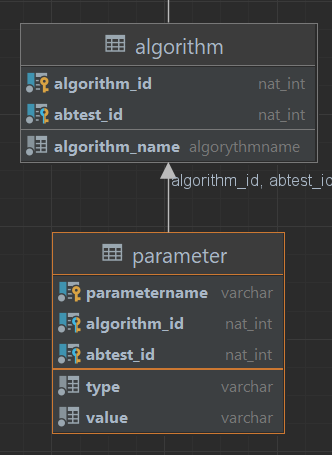
\includegraphics[height={200px}]{Parameter.png}

\end{center}		
	\subsection{Statistics}
	Statistics has a primary key in the form of "statistics-id" but a secondary key (abtest-id, algorithm-id, datetime) is also present. Statistics holds the data that is fetched on a given datetime. One entity of statistics is kept per stepsize.
	\subsubsection{Customer-Specific}
	Here we keep an entry with customer specific data for every customer that has been active (bought something) on the datetime present in statistics. Customer-specific is a weak entity with of statistics with PK(statistics-id,customer-id). It basically links statistics with customer without copying the fields of statistics mindlessly. The customer in it's turn is linked with the dataset(dataset-name)
	
	\subsubsection{recommendation}
	A recommendation entity is kept for every recommendation, this table links the customer-specific statistics with the recommendation-id Which goes up to k-1 in a top-k scenario. It is a weak entity of customer-specific. Its PK = [recommendation-id, customer-id, statistics-id]. It has a foreign key to it's stronger entity customer-specific and article. It can be traced back to the "recommendation-id"th recommendation of customer "customer-id" at (next are linked via statistics-id) "datetime" from algorithm "algorithm-id" in abtest "abtest-id". And even further to dataset and parameters if needed.  
	\begin{center}

		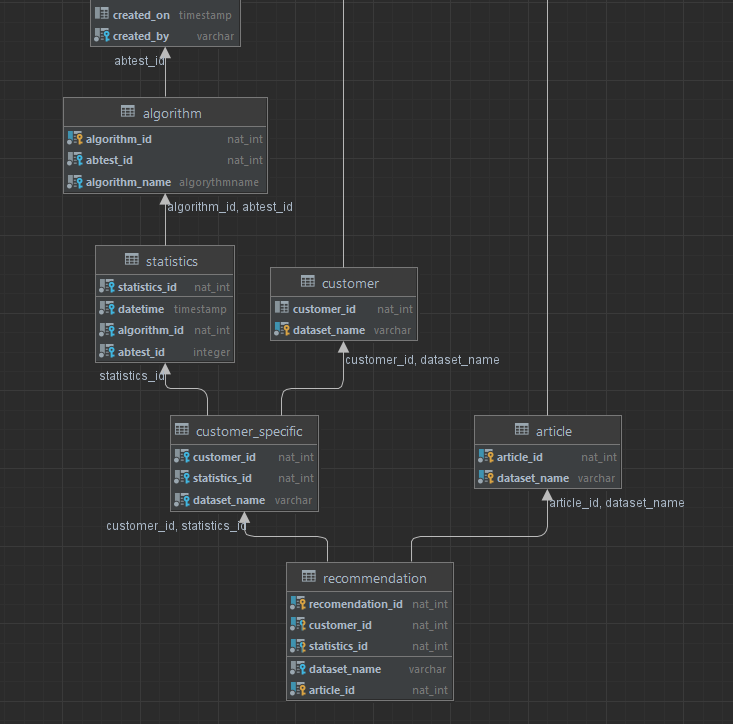
\includegraphics[height={300px}]{Customer-Specific.png}

\end{center}		
\section{Metrics}
Datetime is available in the table of statistics and all dependencies so it is accessible and can be used to chose a window size.
\subsection{Purchases}
Can be done using a simple query: \\
	Select Count(*)\\
	From purchase;\\
\subsection{Active Users}
Can be done using a simple query: \\
	Select COUNT (DISTINCT amount) \\
	FROM	customer\_specific; 
\vspace{15mm}

The following can be done using queries in our database but the exact sql of our queries remains to be seen and decided.
\subsection{Click Through Rate (CTR)}
We know all the purchases that have been made and all the top-k list so we can figure out the click through rate
\subsection{Attribution Rate (AR@D)} 
We can take an intersection of purchases and recommendations, we can see divide the count of purchases with this intersection over a period of 7 or 30 days.
\subsection{Average Revenue Per User (ARPU@D)}
We use the price instead and divide by the amount of active users over the window instead of 7 or 30 days.

\end{document}
